\subsection{GPS Test}
\label{app:gps_test}
\subsubsection*{Introduction}
\vspace{-.3cm}
A test is performed to verify that the positioning provided by the GPS receiver is precise enough to fit the requirements from the control system. All three axes (latitude, longitude, altitude) are tested. Note that the defined requirement regarding the accuracy of the GPS data (P.10) exceeds our needs. See further discussion regarding this point in the discussion subsection. 

This test is performed during a car ride from Skärgårdsstad to Grebbestad on the east and west coasts of Sweden respectively.

\subsubsection*{Method \& Setup}
\vspace{-.3cm}
The GPS receiver is connected to a Raspbery Pi 4B (RPi) and the antenna is taped to the window of the car as shown in figure \ref{gps_pos}. All output from the receiver is logged during the entire journey and saved for analysis.

\begin{figure}[H]
	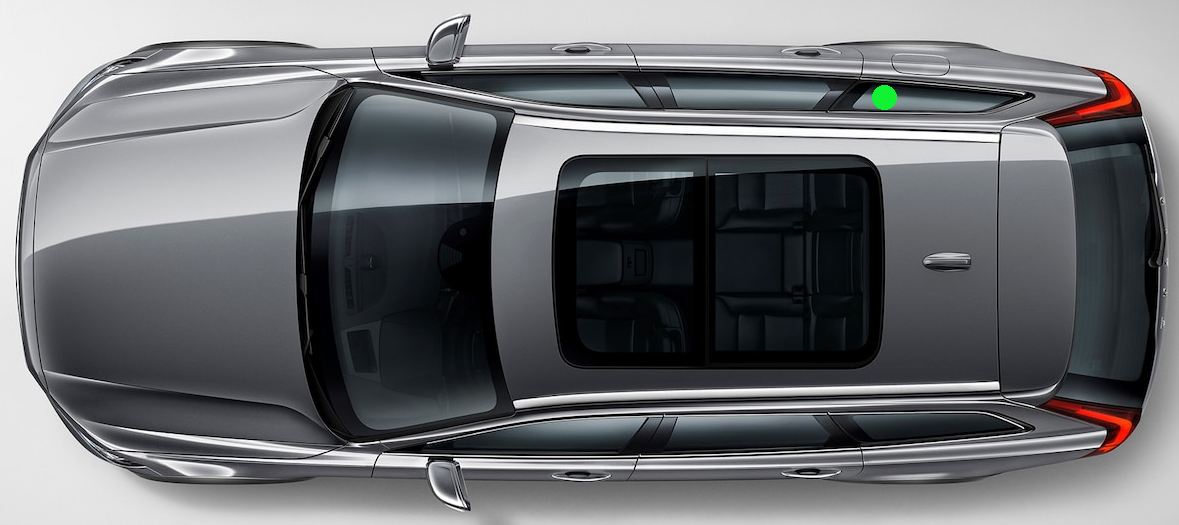
\includegraphics[width=\textwidth]{appendix/img/test-results/gps_pos.png}
	\caption{The green dot shows the position of the gps receiver on the car.}
	\label{gps_pos}
\end{figure}

Due to the lack of access to matching GPS data that is known to be accurate, the latitude and longitude data is plotted in Google MyMaps and compared with satellite imaging. Reference altitude data is produced by \url{https://www.gpsvisualizer.com/elevation} from NASA SRTM1 observational data by fetching altitude from measured latitude and longitude data.

\subsubsection*{Result}
\vspace{-.3cm}
\paragraph{Horizontal Position}
The GPS data plotted on Google MyMaps can be found here: \href{https://drive.google.com/open?id=1pnCSIn2Zt-UFfs62nne9t4oyZEai1yfZ&usp=sharing}{link}. There are three breaks in the data set due to periods where the car engine was off. Data collection during this time was not possible due to the RPi being powered by the car (and the car having a stupid ignition system). \\

As the analysis isn't numerical, an exact accuracy verification cannot be achieved. However, the data points rarely stray off of the roads and if so then only by a few meters on the right side of the road, which is to be expected as the receiver was placed on the right side of the car. Assuming the satellite imaging provided by Google is correct, the horizontal error can be roughly estimated to be within 5 meters.

\paragraph{Vertical Position}

Figure \ref{alt_comp} shows the difference between the measured and generated altitude (measured - generated). This is distributed around -5.7\,m with a standard deviation of 5.2\,m. The magnitude of the largest error encountered is 36.1\,m. Figure \ref{alt_plot} shows both sets of altitude data along the traveled path.

\begin{figure}[H]
	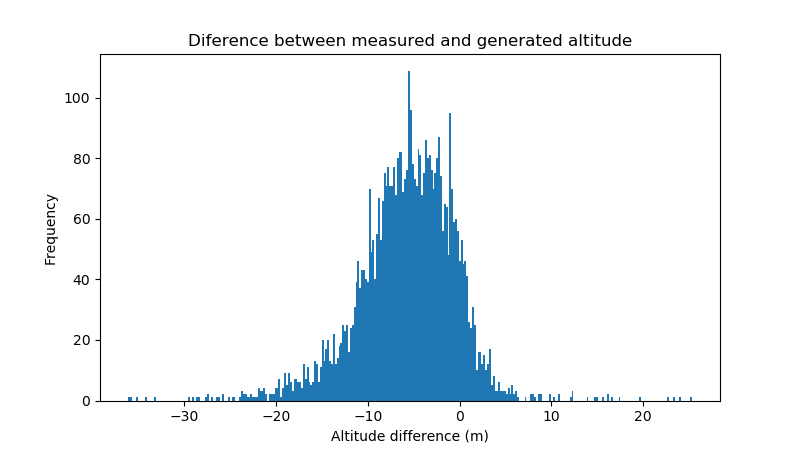
\includegraphics[width=\textwidth]{appendix/img/test-results/gps_alt_comp.png}
	\caption{The distribution of the difference measured - generated altitude.}
	\label{alt_comp}
\end{figure}

\begin{figure}[H]
	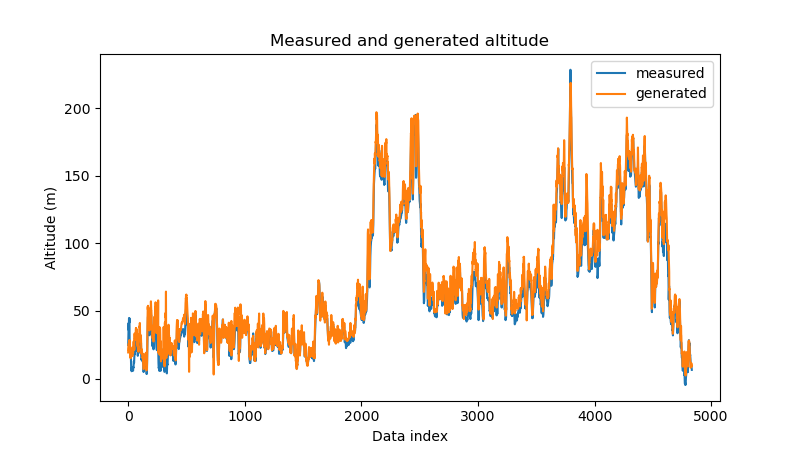
\includegraphics[width=\textwidth]{appendix/img/test-results/gps_alt_plot.png}
	\caption{The altitude along the path as measured and generated data.}
	\label{alt_plot}
\end{figure}

\subsubsection*{Discussion}

The GPS data is mainly required for two things: calculating the sidereal time of the gondola, and monitoring the altitude. An accuracy of 5 meters for either of these purposes is very small. An error one order of magnitude greater would have a minimal effect on any further calculations. For this reason, the requirement specified in the SED is ignored and the accuracy of GPS receiver is deemed to be adequate.\\

There is a bug in the current implementation of the GPS system. If the receiver doesn't have the correct message type ready (GGA) the GPS poller becomes a blocking wait, causing unnecessary usage of system resources. However this bug has only occurred during a hardware error, e.g. one pin disconnecting or a clock speed error (upgrading from the RPi 3B+ to the RPi 4B increases CPU clock speed while using the same library which causes the SPI delay times to be too short). The test described above can also act as an endurance test of roughly 6 hours in total during which this error didn't occur.